\documentclass[12pt]{article}
\usepackage[utf8]{inputenc}
\usepackage{graphicx}
\usepackage{amsmath}

\title{DD Lab 10 Assignment}
\author{Sai Kartik \\2020A3PS0435P}

\begin{document}
\maketitle
\section{Circuit diagram}
\begin{center}
    \begin{figure}[ht]
        \centering
        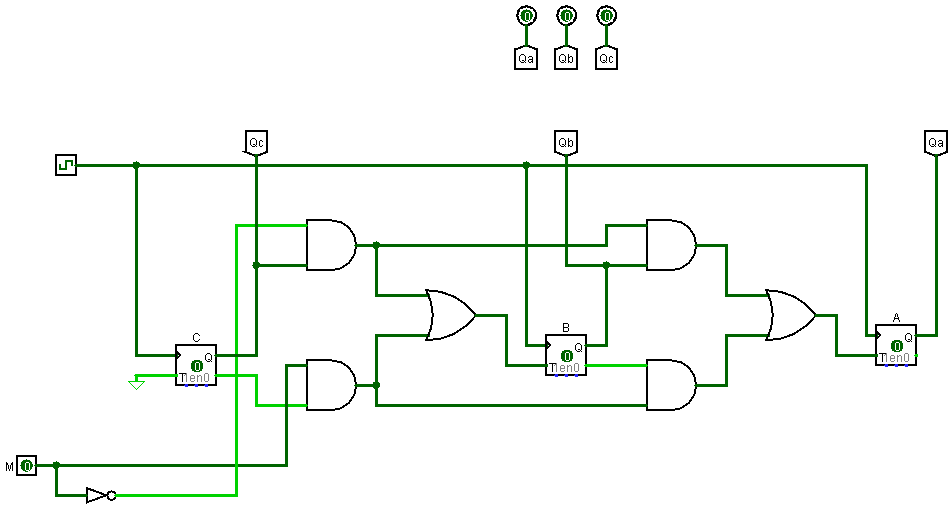
\includegraphics[scale=0.50]{zero.png}
        \caption{Counter at 0}
    \end{figure}
\end{center}
\section{Equations of the flip-flops}
\begin{equation}
    \label{eq:flipflop}
    \begin{cases}
        T_c=1                                 \\[1ex]
        T_b=\bar{M}Q_c+\bar{Q_c}M             \\[1ex]
        T_a=\bar{M}Q_bQ_c+\bar{Q_b}\bar{Q_b}M \\[1ex]
    \end{cases}
\end{equation}
\section{Counter counting up from 0}
\begin{center}
    \begin{figure}[ht]
        \centering
        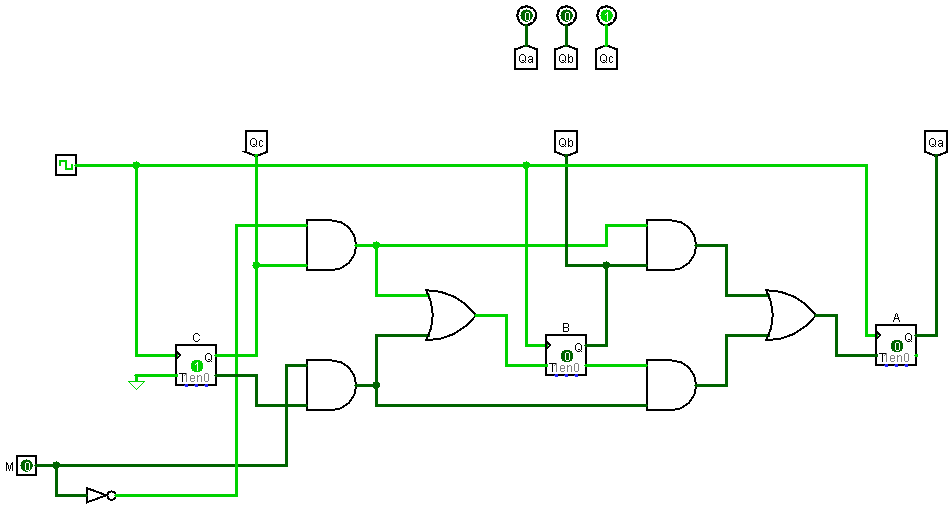
\includegraphics[scale=0.50]{one.png}
        \caption{Counter at 1}
    \end{figure}
\end{center}
\newpage
\section{Counter counting down from 0}
\begin{center}
    \begin{figure}[ht]
        \centering
        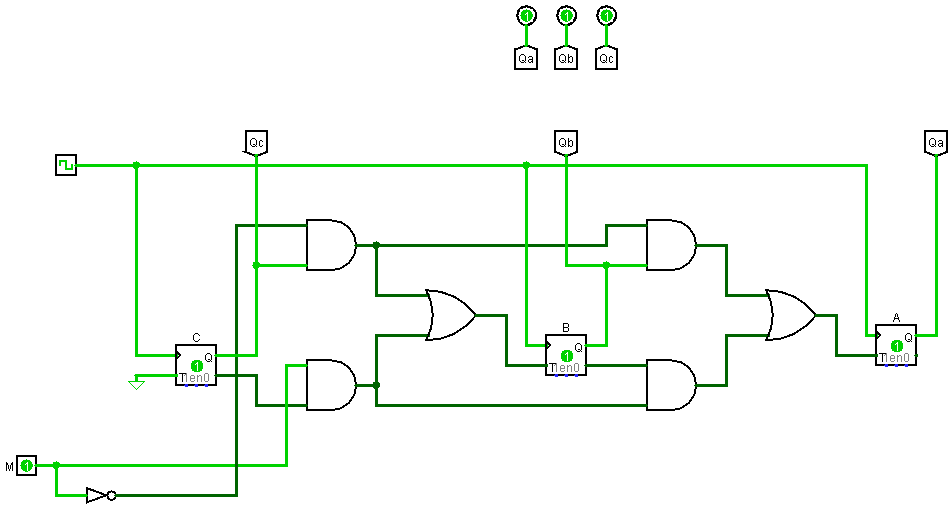
\includegraphics[scale=0.50]{seven.png}
        \caption{Counter at 7}
    \end{figure}
\end{center}
\end{document}
